\newpage

\subsection{Schnittstellenbeschreibung und Integration der Komponenten}
\begin{itemize}
    \item Planung der Schnittstellen zwischen den Komponenten
    \item Einfaches Diagramm in DrawIO:
    \begin{itemize}
        \item Zwischen Jonas und Leon: \texttt{downsampleandread1024()}
        \item Zwischen Syzmon und Jonas: \texttt{filemanager struct}, etc.
        \item Zwischen Szymon und Leon: \texttt{filemanager struct}
    \end{itemize}
    
    
    Folgendes Diagramm zeigt die Relation und Interaktion der 4 Komponenten miteinander.
    
    \begin{figure}[H]
    	\centering
    	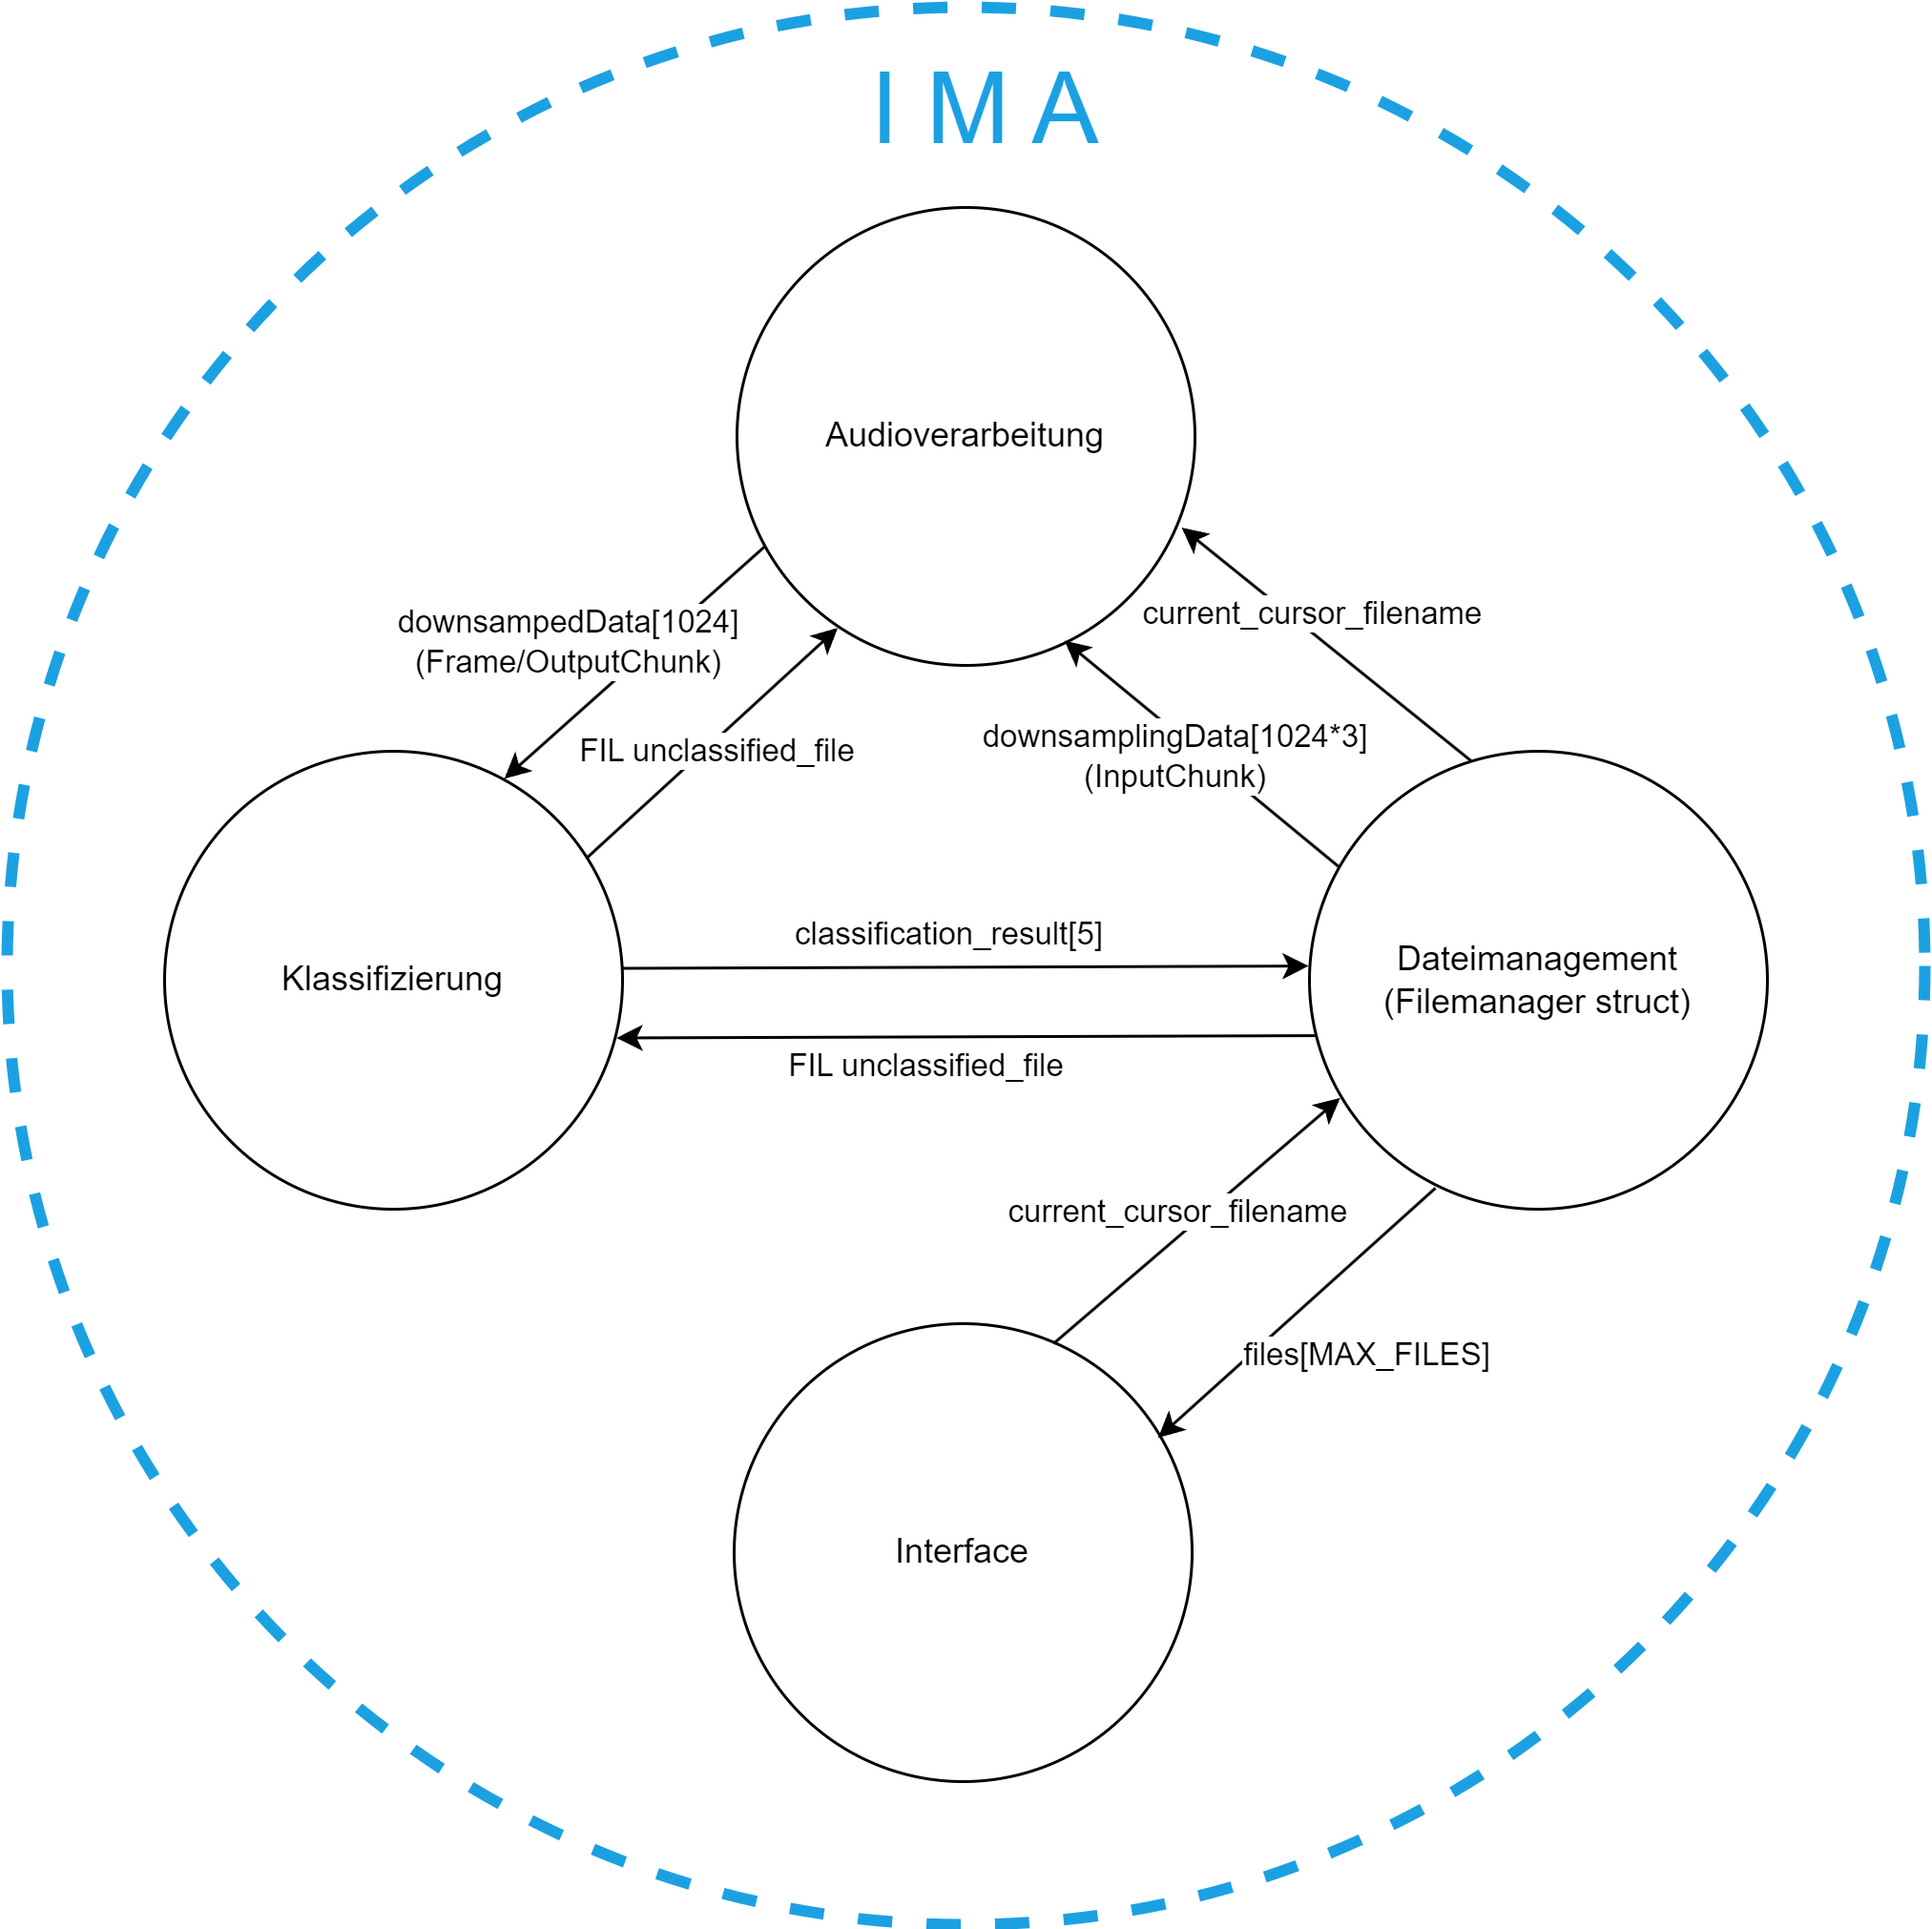
\includegraphics[width=1.0\textwidth]{images/04_spezifikation/komponentendiagramm.drawio.png}
    	\caption{Komponentendiagramm}
    	\label{fig:komponentendiagramm}
    \end{figure}
    
\end{itemize}

Das Dateimanagement ist der zentrale Knotenpunkt des Gesamtsystems. Es dient zunächst als Zugriffspunkt auf die Samples anhand ihrer Namen. 

Beim Hinzufügen neuer \textbf{Samples} in das Dateisystem werden diese zunächst als \boldinline{unclassified_file Fil} an die \boldinline{Klassifizierung} übergeben. Dieser wird an die Audioverarbeitung weiter gegeben. 
 
Diese gibt ein \boldinline{classification_result[5]} zurück, welcher den Dateien zugeordnet wird.

